\part{Modelos implementados y análisis de resultados}
\label{part:explicacionmodelos_analisisrresultados}

\chapter{Modelos implementados}
\label{chapter:modelos}

En este capítulo vamos a repasar los modelos implementados que analizaremos. La implementación de todos estos modelos se ha hecho de forma propia en Python empleando el framework Keras para la construcción de las redes neuronales sobre Tensorflow en su versión 2.

La implementación de todos estos modelos es libre y se puede consultar en el repositorio Deep Learning Outlier Detection o DLOD \href{https://github.com/nacheteam/DLOD}{(link)}.

Para el uso práctico en esta cuestión se han implementado dos tipos de modelos: autoencoders y modelos predictivos. Vamos a repasar brevemente cómo emplearemos estos modelos para la detección de anomalías.

En primer lugar tenemos los modelos Autoencoders, de los que acabamos de hacer un repaso en el capítulo anterior. Los modelos implementados siempre intentan reducir la dimensión para luego reconstruir los datos. Cuando hacemos este paso a un espacio de menor dimensión, estamos intentando reducir las características de nuestras instancias al menor número posible de ellas que las explica lo mejor posible. Nuestra intención al hacer esto es que, las características con las que nos quedamos explican la mayoría de los datos o lo que es lo mismo, los datos normales. Estas características de la reducción de dimensionalidad no van a ser capaces de explicar los datos anómalos y por tanto el error de reconstrucción para los datos anómalos será mayor que el error de reconstrucción para los normales, por lo que podemos usar esta métrica como puntuación o score de anomalía.

En segundo lugar se han implementado modelos de predicción. Estos modelos son entrenados para predecir las secuencias o instancias de datos normales, por lo que aprendemos la distribución subyacente a los datos no anómalos. Cuando intentemos predecir una nueva secuencia de datos normales cometeremos poco error, porque hemos enseñado a nuestra red a que prediga las secuencias normales. Por contra, cuando nos encontremos con datos anómalos, el predictor no tendrá la distribución subyacente de dichos datos y por tanto cometerá mucho más error en la predicción. Teniendo esto podemos usar como métrica o score de anomalía la diferencia entre el dato real y el predicho: a mayor diferencia más anómalo y a menor diferencia menos anómalo.

\section{Autoencoder totalmente conectado}

La primera aproximación lógica sin tener en cuenta el tipo de dato con el que tratamos es un autoencoder con capas densas o totalmente conectadas. El objetivo de este Autoencoder es reconstruir instancia por instancia sin tener en cuenta ningún tipo de temporalidad, como si fuesen datos estáticos. 

Es claro que este tipo de modelos no aprovechan la estructura y dependencia de los datos, pero debemos empezar por algún sitio a probar.

La arquitectura de estos modelos ya ha sido puesta como ejemplo en las secciones anteriores, por lo que no hay mucho más que añadir sobre la misma. En un principio la arquitectura de Autoencoder no tiene por qué ser simétrica, es decir, no tiene por qué ser igual la reducción desde los datos originales al encoding que desde el encoding a la reconstrucción. En el caso que contemplamos se ha utilizado una estructura simétrica, pues es la más empleada y descrita en la literatura.

Para entrenar el autoencoder debemos entrenarlo con datos en condiciones normales para que aprenda bien la distribución subyacente de dichos datos, pues es lo que nos interesa para que el error de reconstrucción sea bajo en los datos normales y alto en los anómalos. En el conjunto de datos del que disponemos, los operarios etiquetan los mantenimientos de la máquina y las alarmas de la misma. Un mantenimiento es precedido por alarmas que no precisan de una parada completa de la misma, mientras que un mantenimiento es un fallo de mayor gravedad que sí requiere de una parada completa para ser solucionado. Este tipo de mantenimientos son los que nos interesan, pero las alarmas nos pueden alertar con anticipación de la ocurrencia de un mantenimiento. Por ello para entrenar el autoencoder se eliminan los datos de mantenimiento y de alarmas, para entrenar siempre la red con datos en condiciones normales.

Para tener un poco más clara la estructura de estas redes vamos a poner un esquema de ejemplo de un posible autoencoder con las dimensiones reales de los datos:

\begin{figure}[H]
	\centering
	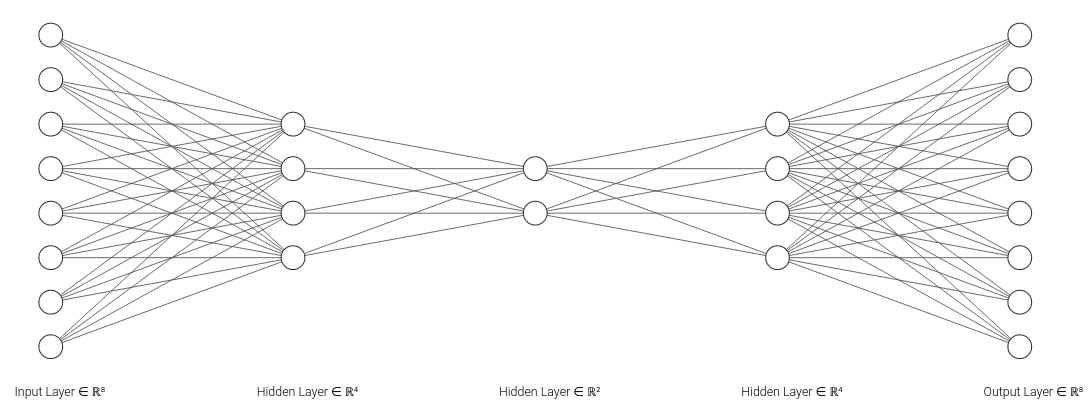
\includegraphics[scale=0.35]{imagenes/autoencoder-fcc.png}
	\caption{Ejemplo de una arquitectura simétrica de autoencoder no completo para detección de anomalías.}
	\label{img:autoencoder-fcc}
\end{figure}

En nuestro caso los datos parten de dimensión 106 (tienen 106 variables numéricas originalmente) y se reducen a 64, 32, y finalmente a 16 características, por lo que se reducen más de 7 veces con respecto a su tamaño original.

Finalmente vamos a ver el código que genera el modelo en Python para terminar esta sección:

\begin{lstlisting}[language=Python]
def buildAutoencoder(self):	
	encoding_dim=self.hidden_neurons[-1]
	
	input_layer = layers.Input(shape=self.input_dim)
	encoder = layers.Dense(self.hidden_neurons[0], activation=self.hidden_activation, activity_regularizer = l2(self.l2_regularizer))(input_layer)
	encoder = layers.Dropout(self.dropout)(encoder)
	
	for neuron in self.hidden_neurons[1:]:
		encoder = layers.Dense(neuron, activation=self.hidden_activation, activity_regularizer = l2(self.l2_regularizer))(encoder)
		encoder = layers.Dropout(self.dropout)(encoder)
	
	reverse_layers = self.hidden_neurons[::-1][1:]
	
	decoder = layers.Dense(reverse_layers[0], activation=self.hidden_activation, activity_regularizer = l2(self.l2_regularizer))(encoder)
	decoder = layers.Dropout(self.dropout)(decoder)
	
	for neuron in reverse_layers[1:]:
		decoder = layers.Dense(neuron, activation=self.hidden_activation, activity_regularizer = l2(self.l2_regularizer))(decoder)
		decoder = layers.Dropout(self.dropout)(decoder)
	
	decoder = layers.Dense(self.input_dim[0], activation=self.output_activation, activity_regularizer = l2(self.l2_regularizer))(decoder)
	
	autoencoder = Model(input_layer, decoder)
	autoencoder.compile(optimizer=self.optimizer, loss=self.loss)
	
	return autoencoder
\end{lstlisting}

Cabe decir que esta función está encapsulada dentro de una clase que se encarga de generar la estructura en base a unos parámetros, entrenarla con los datos que le demos al modelo y predecir y sacar la puntuación de anomalía para cada una de las instancias del conjunto de test.

\section{Autoencoder totalmente conectado por lotes}

En la sección anterior hemos comentado que el primero paso natural al hacer un autoencoder para detección de anomalías es empezar por la arquitectura más sencilla posible: la totalmente conectada. También hemos comentado que esta arquitectura no aprende ni usa la dependencia temporal de los datos presente por ser estos una serie temporal, por tanto es una herramienta de poco potencial para este tipo de datos.

Las capas totalmente conectadas también nos pueden valer para procesar lotes de datos, es decir, bloques de datos sin saltos temporales. De esta forma, podemos hacer que una arquitectura sencilla pueda aprender algo más sobre la dependencia temporal de los datos. Si lo pensamos, lo que estamos haciendo para poder procesar lotes, es tomar $n$ datos juntos y colocarlos en formato columna uno detrás de otro, por lo que nuestro objetivo final ya no será la reconstrucción de una instancia, si no la reconstrucción de un lote completo.

Esto es una aproximación un poco mejor que la anterior, pues ahora ya tenemos datos completos y podemos procesar y aprender la distribución subyacente pero por supuesto no es tan potente como las capas que hemos estudiado en la parte teórica.

En este caso, para que tengamos solo una puntuación por instancia, hemos reconstruido lotes sin solapamiento. Es decir, procesamos las primeras $n$ instancias, luego desde la $n+1$ hasta la $2n$ etcétera. Con esto no tenemos que hacer ponderaciones de las puntuaciones al obtener sólo una por instancia ya que los lotes no contienen datos repetidos.

El esquema de esta arquitectura empieza con un lote de datos en formato matriz, que reconvertimos a un vector colocando una fila detrás de la siguiente. Tras esta conversión de tamaños tenemos la misma arquitectura que en la sección anterior siendo el final la operación inversa de vector a matriz.

\begin{figure}[H]
	\centering
	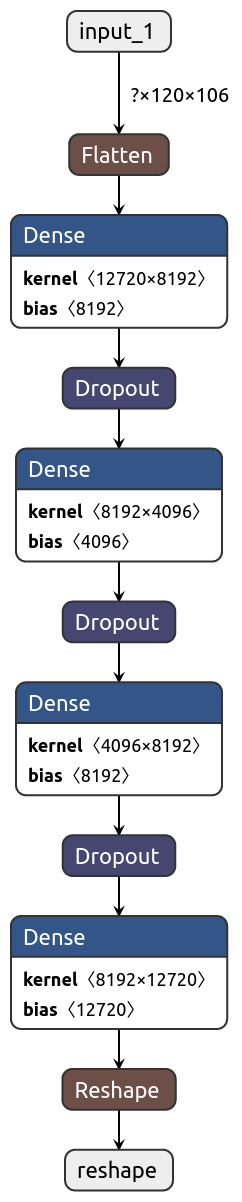
\includegraphics[scale=0.4]{imagenes/autoencoder-fcc-batch.png}
	\caption{Ejemplo de una arquitectura de Autoencoder de reconstrucción por lotes.}
	\label{img:autoencoder-fcc-batch}
\end{figure}

Como podemos ver en la arquitectura, se recibe una matriz de 120 instancias de 106 atributos cada una de ellas y lo primero que hacemos con ella es aplanarla como hemos comentado. Tras esto viene toda la arquitectura normal de un autoencoder no completo para finalizar con un reshape que nos devuelve la salida a un formato matricial.

\begin{lstlisting}[language=Python]
def buildAutoencoder(self):
	encoding_dim=self.hidden_neurons[-1]
	
	input_layer = layers.Input(shape=(self.instance_batch, self.num_features))
	flatten = layers.Flatten()(input_layer)
	encoder = layers.Dense(self.hidden_neurons[0], activation=self.hidden_activation, activity_regularizer = l2(self.l2_regularizer))(flatten)
	encoder = layers.Dropout(self.dropout)(encoder)
	
	for neuron in self.hidden_neurons[1:]:
		encoder = layers.Dense(neuron, activation=self.hidden_activation, activity_regularizer = l2(self.l2_regularizer))(encoder)
		encoder = layers.Dropout(self.dropout)(encoder)
	
	reverse_layers = self.hidden_neurons[::-1][1:]
	
	decoder = layers.Dense(reverse_layers[0], activation=self.hidden_activation, activity_regularizer = l2(self.l2_regularizer))(encoder)
	decoder = layers.Dropout(self.dropout)(decoder)
	
	for neuron in reverse_layers[1:]:
		decoder = layers.Dense(neuron, activation=self.hidden_activation, activity_regularizer = l2(self.l2_regularizer))(decoder)
		decoder = layers.Dropout(self.dropout)(decoder)
	
	decoder = layers.Dense(self.instance_batch * self.num_features, activation=self.output_activation, activity_regularizer = l2(self.l2_regularizer))(decoder)
	reshape = layers.Reshape(target_shape=(self.instance_batch, self.num_features))(decoder)
	
	autoencoder = Model(input_layer, reshape)
	autoencoder.compile(optimizer=self.optimizer, loss=self.loss)
	
	return autoencoder
\end{lstlisting}

\section{Autoencoder LSTM}

La siguiente arquitectura que se ha desarrollado es la última que toma como estructura la de codificación-reconstrucción. En este caso, para poder aprovechar al máximo la dependencia temporal y aplicando lo que hemos visto en la sección de teoría, se ha desarrollado un Autoencoder con capas LSTM. En este caso, como ya hemos visto, las capas LSTM aprovechan la dependencia temporal ya que tienen un estado interno que les permite almacenar información de las instancias anteriores y poder olvidarlo cuando sea necesario.

En este modelo de red podemos construirlo de distintas formas. En primer lugar podemos pensar en un modelo mixto que tenga una primera capa LSTM y luego haga la codificación con las características obtenidas de la capa LSTM a través de capas totalmente conectadas. La otra opción es que hagamos un Autoencoder sólo con capas LSTM, este es el tipo de modelo que se ha elegido. 

La elección de un Autoencoder de capas LSTM únicamente responde a la capacidad de olvidar información que tienen estas capas. Si sólo fuese interesante sacar dependencias temporales en las primeras capas las siguientes estarían activando el olvido y el bloqueo de entrada-salida para forzar a que su funcionamiento sea como el de una capa totalmente conectada con estados internos intermedios. Este razonamiento es el que nos lleva a confiar en la capacidad y potencia de estas capas para elaborar un Autoencoder sólo con ellas.

\begin{figure}[H]
	\centering
	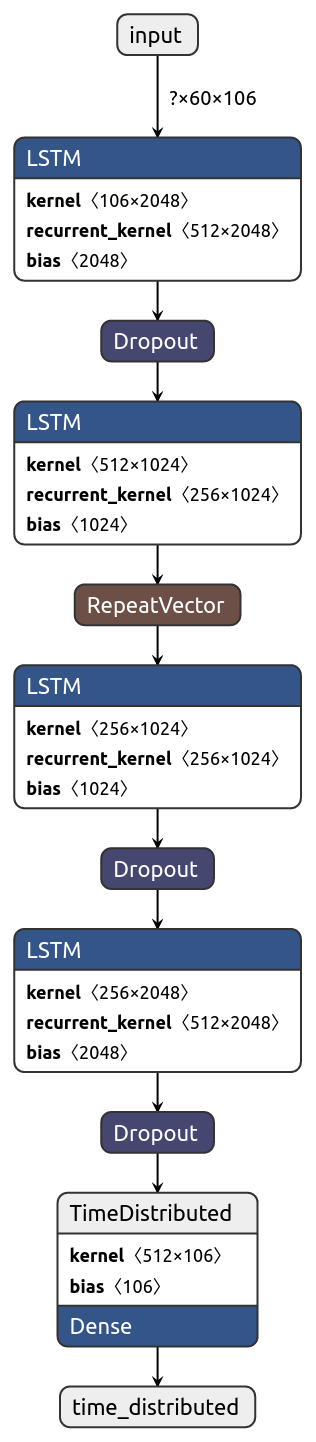
\includegraphics[scale=0.4]{imagenes/autoencoder-lstm.png}
	\caption{Ejemplo de una arquitectura de Autoencoder LSTM.}
	\label{img:autoencoder-lstm}
\end{figure}

Como podemos ver, el modelo de Autoencoder con capas LSTM puede tener varias capas hasta el encoding y respeta la simetría que hemos comentado antes. La programación de este tipo de redes es un poco compleja, pues tenemos que tener en cuanta cuándo tenemos que devolver secuencias de datos y cuándo vectores para que las salidas de una capa encajen con las entradas que espera la siguiente capa.

Para esta arquitectura de red estamos introduciendo un lote de datos, como en el caso de la sección anterior una matriz con varias instancias de datos. Cuando vamos pasando de una capa a otra tenemos que devolver secuencias, pues es lo que las capas LSTM esperan, pero cuando llegamos al encoding queremos obtener un vector como en los otros modelos de encoding. Es por esto que tenemos que repetir ese vector de encoding para poder hacer de nuevo la subida o decoding hacia la reconstrucción de los datos, pues de otra forma no recibirían una secuencia.

Veamos por último el código Python que genera este tipo de modelos:

\begin{lstlisting}[language=Python]
def buildAutoencoder(self):
	autoencoder = Sequential()
	autoencoder.add(layers.InputLayer(input_shape = (self.instance_batch, self.num_features)))
	for neurons in self.hidden_neurons[:-1]:
		autoencoder.add(layers.LSTM(units=neurons,
		activation=self.hidden_activation,
		recurrent_activation=self.recurrent_activation,
		activity_regularizer=l2(self.l2_regularizer),
		recurrent_dropout=self.recurrent_dropout,
		return_sequences=True))
		autoencoder.add(layers.Dropout(self.dropout))
	autoencoder.add(layers.LSTM(units=self.hidden_neurons[-1],
	activation=self.hidden_activation,
	recurrent_activation=self.recurrent_activation,
	activity_regularizer=l2(self.l2_regularizer),
	recurrent_dropout=self.recurrent_dropout,
	return_sequences=False))
	autoencoder.add(layers.RepeatVector(n=self.instance_batch))
	for neurons in self.hidden_neurons[::-1]:
		autoencoder.add(layers.LSTM(units=neurons,
		activation=self.hidden_activation,
		recurrent_activation=self.recurrent_activation,
		activity_regularizer=l2(self.l2_regularizer),
		recurrent_dropout=self.recurrent_dropout,
		return_sequences=True))
		autoencoder.add(layers.Dropout(self.dropout))
	autoencoder.add(layers.TimeDistributed(layers.Dense(units=self.num_features)))
	autoencoder.compile(optimizer=self.optimizer, loss=self.loss)
return autoencoder
\end{lstlisting}

\section{Modelo de predicción LSTM}

Este modelo entra dentro del segundo tipo de modelos implementados: los de predicción. La intención de estos modelos es aprender a predecir muy bien las instancias en momentos de comportamiento normal de la máquina, de esta forma cuando estemos ante datos normales tendremos un error de predicción muy pequeño y cuando estemos ante datos anómalos con los que no se ha entrenado el error será mayor.

Para esta arquitectura se han empleado de nuevo capas LSTM. Con estas capas podemos obtener dependencias temporales de los datos, por lo que el modelo lo que va a hacer es tomar lotes de $n$ datos y predecir los $m$ siguientes. Este número $m$ puede ser uno o puede ser mayor que uno, es decir, con un lote podemos predecir uno o más datos siguientes. En este estudio se ha considerado que la mejor elección y la más precisa es la de predicción punto a punto, es decir, tomamos un lote y predecimos el siguiente punto, desplazamos el lote un instante de tiempo y volvemos a predecir la siguiente instancia. De esta forma lo que tenemos es una única predicción de cada instancia y predecimos solo un dato por cada lote que tenemos. El código desarrollado está preparado para soportar más de una predicción si se considerase necesario.

Debemos tener en cuenta que hacer esta operación de entrenamiento es altamente costosa pues, para poder predecir cada una de las instancias de un conjunto de 40 millones de datos aproximadamente, necesitamos almacenar en memoria $40 \ millones \cdot n$. Si consideramos por ejemplo lotes de 60 instancias o lo que es lo mismo un minuto de datos, tenemos que almacenar en memoria 240 millones de instancias lo cual no es posible. Por ello cabe detenerse un momento en explicar la solución técnica que se ha adoptado para solventar este contratiempo.

Cuando queremos entrenar una red con una serie temporal de un gran tamaño Keras tiene como herramienta la clase TimeSeriesGenerator, que nos permite hacer lotes de series temporales con lo que queremos que entrene y el objetivo al que queremos que llegue. Esta herramienta actualmente tiene un problema, pues sólo permite el uso para predicción con el siguiente punto y no con varias instancias por lote. Aunque para este experimento no se ha empleado esto se ha generalizado el funcionamiento de la clase TimeSeriesGenerator de Keras para que pueda devolver varias instancias por cada lote.

Veamos ahora la estructura de este tipo de redes:

\begin{figure}[H]
	\centering
	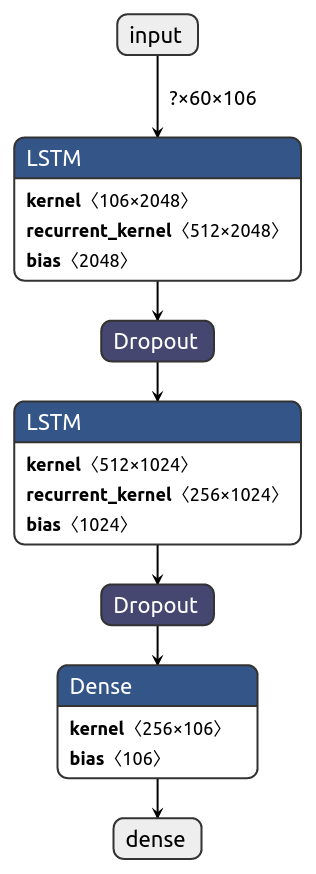
\includegraphics[scale=0.4]{imagenes/lstm-forecaster.png}
	\caption{Ejemplo de una arquitectura de predictor LSTM con una única instancia en la predicción.}
	\label{img:forecaster-lstm}
\end{figure}

Como podemos ver, en este ejemplo tenemos dos capas LSTM y una capa final totalmente conectada. Las capas LSTM nos sirven para poder obtener las dependencias temporales que tenemos intrínsecas por ser series temporales. Estas características son pasadas a una última capa totalmente conectada que nos sirve para igualar la dimensión a la que queramos. En esta red estamos prediciendo una única instancia por batch, pero como es lógico la arquitectura variaría ligeramente, vamos a ver un ejemplo de cómo sería la arquitectura de la red si quisiéramos predecir más de una instancia:

\begin{figure}[H]
	\centering
	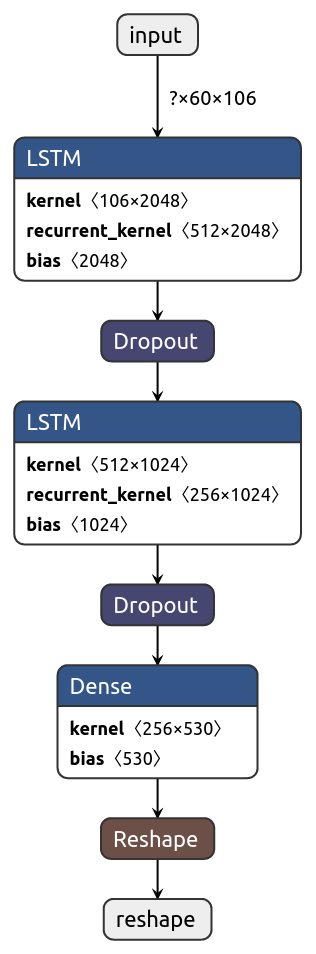
\includegraphics[scale=0.4]{imagenes/lstm-forecaster2.png}
	\caption{Ejemplo de una arquitectura de predictor LSTM con 5 instancias en la predicción.}
	\label{img:forecaster-lstm2}
\end{figure}

Como podemos ver la capa totalmente conectada del final ahora tiene como tamaño la dimensión de los datos por el número de instancias que queremos predecir, por lo que la capa siguiente es una capa de reajuste de los datos que nos los convierte a una matriz en la que cada fila es una de las instancias predichas, yendo estas en orden. Esto quiere decir que la primera fila está temporalmente antes que la segunda y así sucesivamente.

Lo último que queda por añadir es que para entrenar todos estos modelos con secuencias de datos, nos tenemos que asegurar que no son secuencias cortadas. Al eliminar los datos anómalos como las alarmas y los mantenimientos se nos quedan huecos temporales en los datos. Estos huecos pueden producir que haya secuencias con saltos temporales, lo cual no es deseable así que tenemos que eliminar las secuencias que contengan alguno de estos saltos temporales.

Finalmente este es el código que genera este tipo de arquitecturas:

\begin{lstlisting}[language=Python]
def buildForecaster(self):
	model = Sequential()
	model.add(layers.InputLayer(input_shape = (self.instance_batch, self.num_features)))
	for neurons in self.hidden_neurons[:-1]:
		model.add(layers.LSTM(units=neurons,
		activation=self.hidden_activation,
		recurrent_activation=self.recurrent_activation,
		activity_regularizer=l2(self.l2_regularizer),
		recurrent_dropout=self.recurrent_dropout,
		return_sequences=True))
		model.add(layers.Dropout(self.dropout))
	model.add(layers.LSTM(units=self.hidden_neurons[-1],
	activation=self.hidden_activation,
	recurrent_activation=self.recurrent_activation,
	activity_regularizer=l2(self.l2_regularizer),
	recurrent_dropout=self.recurrent_dropout,
	return_sequences=False))
	model.add(layers.Dropout(self.dropout))
	model.add(layers.Dense(self.num_features*self.npred, activation=self.output_activation, activity_regularizer = l2(self.l2_regularizer)))
	if self.npred>1:
		model.add(layers.Reshape(target_shape=(self.npred, self.num_features)))
	model.compile(optimizer=self.optimizer, loss=self.loss)
	return model
\end{lstlisting}

\section{Modelo de predicción CNN-LSTM}

El último modelo implementado es otro modelo de predicción como el se la sección anterior, pero ahora empleamos capas convolucionales para intentar extraer características más relevantes de los datos sin romper la temporalidad de los mismos antes de pasarlos por las capas LSTM.

Lo primero que vamos a hacer con la entrada es pasarla por capas convolucionales 1D. En la sección de teoría estudiamos el comportamiento de estas capas, introduciendo primero la operación de convolución en una dimensión y luego en dos dimensiones. Cuando aplicamos la operación de convolución en dos dimensiones, para que sea útil e interesante, tenemos que tener datos que estén correlados o que tengan dependencias en ambas dimensiones. Si pensamos por ejemplo en una imagen, es claro que la información de un píxel está condicionada por la de los píxeles que tiene a su alrededor. En el caso que tenemos nosotros no es así. Tenemos una matriz cuyas filas son cada una de las instancias consideradas y las columnas son las características de dichas instancias. Es claro que tenemos una dependencia en el eje Y, es decir entre las filas, pues las instancias están consecutivas en el tiempo y cada una de ellas está condicionada por las anteriores y condiciona las siguientes. Por contra, en las columnas, no tenemos esa dependencia. A priori las características no tienen ningún tipo de dependencia entre sí ni correlación, pues no se han ordenado para ello ni tendría por qué existir dicha correlación entre las variables si tenemos un conjunto de datos óptimo.

Con esto dicho por tanto está claro el eje en el que tiene sentido hacer la convolución: el eje de las filas. Este tipo de operación de convolución uno dimensional está soportada por Keras mediante la capa Conv1D. Tras pasar los datos por varias convoluciones y agregaciones se pasan por capas LSTM, de forma que con las nuevas características obtenidas por la convolución las capas LSTM pueden trabajar algo mejor. Finalmente la arquitectura de la red termina con una serie de capas totalmente conectadas que igualan la dimensión con la que nosotros queramos para predecir una o más instancias.

Estos modelos son ampliamente empleados en predicción por su buen desempeño como se puede ver en los artículos \cite{lih_oh_automated_2018} y \cite{tae_young_predicting_2019} que han servido para obtener una arquitectura de red adecuada para nuestro problema.

En cuanto al entrenamiento y predicción este modelo es muy similar al anterior. Vamos a entrenarlo con secuencias de datos y vamos a predecir una única instancia, aunque el modelo está preparado en su implementación para poder predecir más de una por cada lote. Además, nos aseguramos también de que el modelo no se entrena con secuencias de datos con saltos temporales. De igual forma es necesario emplear la clase TimeSeriesGenerator modificada para poder manejar los datos de entrenamiento, pues al predecir una instancia por lote tenemos muchos más datos que los originales.

Veamos un esquema de este tipo de arquitectura:

\begin{figure}[H]
	\centering
	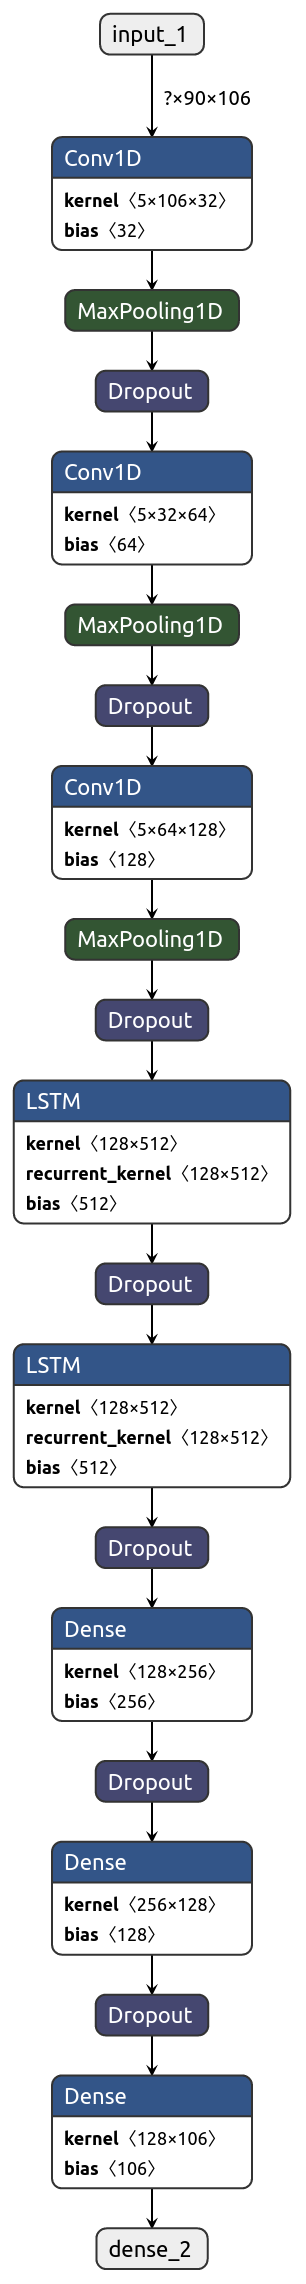
\includegraphics[scale=0.28]{imagenes/cnn-lstm-forecaster.png}
	\caption{Ejemplo de una arquitectura de predictor CNN-LSTM.}
	\label{img:cnn-lstm-forecaster}
\end{figure}

Como podemos ver en este ejemplo tenemos tres capas de convolución con 3 agregaciones con el máximo, tras esto dos capas LSTM y finalmente otras dos capas totalmente conectadas que hacen que la dimensión final sea la de una instancia, por lo que este ejemplo en concreto predice una única instancia. Si quisiéramos predecir más de una tendríamos que hacer lo mismo que en el modelo anterior, añadiendo un reshape.

Por último veamos el código Python que genera el modelo:

\begin{lstlisting}[language=Python]
def buildForecaster(self):
	input = layers.Input(shape = (self.instance_batch, self.num_features))
	
	conv = layers.Conv1D(filters=self.conv_filters[0], kernel_size = self.kernel_size,
	activation=self.conv_activation)(input)
	conv = layers.MaxPooling1D(self.pooling_size)(conv)
	conv = layers.Dropout(self.dropout)(conv)
	for nfilters in self.conv_filters[1:]:
		conv = layers.Conv1D(filters=nfilters, kernel_size = self.kernel_size,
		activation=self.conv_activation)(conv)
		conv = layers.MaxPooling1D(self.pooling_size)(conv)
		conv = layers.Dropout(self.dropout)(conv)
	
	lstm=None
	first_lstm=True
	for neurons in self.lstm_neurons[1:]:
		if first_lstm:
			lstm = layers.LSTM(units=neurons,
			activation=self.lstm_activation,
			recurrent_activation=self.recurrent_activation,
			activity_regularizer=l2(self.l2_regularizer),
			recurrent_dropout = self.recurrent_dropout,
			return_sequences=True)(conv)
			lstm = layers.Dropout(self.dropout)(lstm)
			first_lstm=False
		else:
			lstm = layers.LSTM(units=neurons,
			activation=self.lstm_activation,
			recurrent_activation=self.recurrent_activation,
			activity_regularizer=l2(self.l2_regularizer),
			recurrent_dropout = self.recurrent_dropout,
			return_sequences=True)(lstm)
			lstm = layers.Dropout(self.dropout)(lstm)
	lstm = layers.LSTM(units=neurons,
	activation=self.lstm_activation,
	recurrent_activation=self.recurrent_activation,
	activity_regularizer=l2(self.l2_regularizer),
	recurrent_dropout = self.recurrent_dropout,
	return_sequences=False)(lstm)
	lstm = layers.Dropout(self.dropout)(lstm)
	
	dense=None
	if len(self.dense_neurons)>1:
		dense = layers.Dense(units=self.dense_neurons[0], activation=self.dense_activation)(lstm)
		dense = layers.Dropout(self.dropout)(dense)
	for neurons in self.dense_neurons[1:]:
		dense = layers.Dense(units=neurons, activation=self.dense_activation)(dense)
		dense = layers.Dropout(self.dropout)(dense)
	
	if len(self.dense_neurons)==0:
		dense = layers.Dense(units=self.num_features, activation=self.output_activation)(lstm)
	else:
		dense = layers.Dense(units=self.num_features, activation=self.output_activation)(dense)
	
	model = Model(inputs=input, outputs=dense)
	model.compile(optimizer=self.optimizer, loss=self.loss)
	return model
\end{lstlisting}